%%%%%%%%%%%%%%%%%%%%%%%%%%%%%%%%%%%%%%%%%%%%%%%%%%%%%%%%%%%%%%
%% LaTeX template for the science justification to be       %%
%%       submitted as part of an ALMA proposal.             %%
%%                                                          %%
%%                      ALMA Cycle 3                        %%
%%                                                          %%
%%%%%%%%%%%%%%%%%%%%%%%%%%%%%%%%%%%%%%%%%%%%%%%%%%%%%%%%%%%%%%

%%%%%%%%%%%%%%%%%%%%%%%%%%%%%%%%%%%%%%%%%%%%%%%%%%
%%%%% How to convert this document to PDF %%%%%%%%
%%%%%%%%%%%%%%%%%%%%%%%%%%%%%%%%%%%%%%%%%%%%%%%%%%

% If your figures are stored as PostScript files, you can use the 
% following commands to generate a PDF file of your proposal:

%% latex file.tex
%% dvips file.dvi
%% ps2pdf file.ps file.pdf 


% If your figures are PDF images or bitmap pictures in PNG, JPG, or GIF format,
% you can use the pdflatex command to generate a PDF file from this template
% (note, however, that the pdflatex command does not handle PostScript files):

% pdflatex file.tex


% WARNINGS: 
%           1. You must make sure that PDF output generated from this
%              template is complete both when displayed with a viewer 
%              (acroread, for example) and when printed on paper.
%              LaTeX installations vary greatly and therefore it might 
%              not be possible to get all proposals to come out 
%              correctly with a single text page layout. 
%              In some cases you will have to adjust the 
%              \topmargin=-7mm command in the template to center the 
%              text vertically in the page.  
%           2. The scientific justification, figures, tables, references,
%              and public outreach statement must all fit within the
%              4-page limit.
%           3. You are free to include colour images in your proposal 
%              justification. Proposals are distributed to ALMA Review Panels 
%              in electronic form. However, the scientific content of the 
%              images should still remain clear when displayed or printed
%              in black and white.

%%%%%%%%%%%%%%%%%%%%%%%%%%%%%%%%%%%%%%%%%%%%%%
%%%%% Default format: 12pt single column %%%%%
%%%%%%%%%%%%%%%%%%%%%%%%%%%%%%%%%%%%%%%%%%%%%%

\documentclass[12pt,a4paper]{article}
%11pt is smallest allowed

\usepackage{graphics,graphicx}
\usepackage{wrapfig}
\usepackage{amssymb}
\usepackage{color}
\definecolor{tan}{rgb}{0.96,.92,0.83}
\usepackage[textsize=scriptsize]{todonotes}
\usepackage{multicol}
\usepackage{caption}
\usepackage{hyperref}

\newcommand{\herschel}{{\it Herschel}}
\newcommand{\hermes}{HerMES}
\newcommand{\atlas}{H-ATLAS}
\newcommand{\spitzer}{{\it Spitzer}}
\newcommand{\chandra}{{\it Chandra}}
\newcommand{\fermi}{{\it Fermi}}
\newcommand{\ea}{et~al.}
\newcommand{\hst}{{\it HST}}
\newcommand{\myr}{${\rm M_{\sun}yr^{-1}}$}
\newcommand{\lsun}{${\rm L_{\sun}}$}
\newcommand{\zphot}{z_{\rm phot}}
\newcommand{\hyperz}{{\sc Hyperz}}
\newcommand{\ujy}{$\mu$Jy}
\newcommand{\micron}{$\mu$m}
\newcommand{\arcsec}{$^{\prime\prime}$}
\newcommand{\mumax}{$\mu_{\rm max}$}
\newcommand{\bootes}{Bo\"{o}tes}
\newcommand{\eyelash}{SMMJ2135$-$0102}
\newcommand\sun{\odot}

%%%%%%%%%%%%%%%%%%%%%%%%%%%%
%%%%%% Page dimensions %%%%%
%%%%%%  DO NOT CHANGE  %%%%%
%%%%%%%%%%%%%%%%%%%%%%%%%%%%

\textheight=247mm
\textwidth=180mm
%\topmargin=-7mm
\topmargin=-25mm
\oddsidemargin=-10mm
\evensidemargin=-10mm
\parindent 10pt

%%%%%%%%%%%%%%%%%%%%%%%%%%%%%
%%%%% Start of document %%%%% 
%%%%%%%%%%%%%%%%%%%%%%%%%%%%%

\begin{document}
\pagestyle{plain}
\pagenumbering{arabic}
 
%%%%%%%%%%%%%%%%%%%%%%%%%%%%%
%%%%% Title of proposal %%%%%
%%%%%%%%%%%%%%%%%%%%%%%%%%%%%

\begin{center}
{\LARGE{\bf
%%
%% ENTER TITLE OF PROPOSAL BELOW THIS LINE
{Resolving the Herschel-SPIRE confusion}
%%
%%
}}
\end{center}
%\bigskip

%% Principal Investigator (PI) initial(s) and family name %%
\centerline{\bf PI: 
%% ENTER NAME OF PI BELOW THIS LINE
{Julie Wardlow}}
%%   
%%   \bigskip
%%   
%%   % Type a concise abstract of your proposal here (optional).
%%   
%%   \section{Abstract}
%%   Include here the abstract of your proposal (optional)

%%%%%%%%%%%%%%%%%%%%%%%%%%%%%%%%%%%%%%%%%
%%%%% Body of science justification %%%%%
%%%%%%%%%%%%%%%%%%%%%%%%%%%%%%%%%%%%%%%%%

%% ENTER TEXT, FIGURES AND TABLES BELOW

{\large{\bf1 Scientific Justification}}

{\bf Summary: }
%
The Cosmic Infrared Background (CIB; Puget et al.\ 1996; Fixsen et
al.\ 1998; Lagache et al.\ 1999) has an intensity roughly equal to the
Cosmic Optical Background, signifying that $\sim$ half of stellar
and AGN emission has been
reprocessed by dust (Hauser \& Dwek 2001; Dole et al.\ 2006). Thus, to
reveal the 50\% of energy generation in the Universe that is dust-obscured, and
its role in galaxy evolution, it is imperative that we study the dusty
sources that comprise the CIB. It appears that the peak is dominated by star forming galaxies at redshift 1--2. \herschel\ detects galaxies whose emission peaks at this wavelength and are thus representative of the most luminous contributors to the CIB, providing important insights into these populations, challenging theories. However, these \herschel\ studies are compromised by poor partial resolution.  
%
This program will observe band 7 continuum
emission for 300 \herschel-SPIRE sources with $S_{250}>35$mJy, in the COSMOS field.
\indent\indent\colorbox{tan}{
\begin{minipage}{16cm}
\noindent Our key science goals are to:

$\bullet$ Use the resolution of ALMA to reliably pin-point the galaxies
that contribute to the \herschel\ emission, and definitively identify
their multi-wavelength counterparts in existing ancillary data.

%$\bullet$ Assess the success, or otherwise, of statistical methods of
%identifying \herschel-SPIRE sources. Determine the completeness and
%reliability of methods that attempt to deblend these sources with
%prior (typically shorter wavelength) multiwavelength information
%(e.g.\ Roseboom \ea\ 2010, 2012, Hurley \ea in prep.).

$\bullet$ Measure the redshift, dust temperature, infrared luminosity,
stellar mass, and AGN contribution of 250-\micron\
selected sources by combing the ALMA positional and flux information
with the extensive archival data in COSMOS.

$\bullet$ Derive fundamental constraints on models of galaxy formation
by comparing predictions with our complete redshift, far-infrared
luminosity, temperature and stellar mass distributions for
250-\micron\ selected sources.

\end{minipage}}

%\vspace{0.3cm}
{\bf The importance of \herschel\ selected samples: }
%
%The CIB peaks at $\sim$200\micron\ (Dole et al.\ 2006) so analyses of
%the contributors selected at wavelengths around this peak are
%central to understanding the role of dust-obscured sources in the
%history of galaxy formation and evolution. Samples selected at longer wavelengths (e.g.\ 850\,\micron,
%1.1\,mm) only have minimal overlap 
%with the galaxies that contribute to the peak of the CIB, and are biased towards the higher redshift galaxies, whilst samples at shorter wavelengths (e.g. \ 24, 100\,\micron) are biased towards warmer and/or lower redshift galaxies.

At 250\,\micron\,, \herschel-SPIRE observations provide an unbiased selection of objects which significantly contribute to the peak of the CIB $\sim$200\micron\ (Dole et al.\ 2006) thus measuring the bolometric power whilst not biasing to warmer (q.v. \spitzer) or cooler galaxies (q.v. {\it SCUBA}).  \herschel-SPIRE is also the premier instrument for
wide-field extragalactic surveys at around the peak of the CIB because it has the
resolution, sensitivity and mapping speeds to resolve a substantial
fraction of the CIB in
uniform wide-field surveys (e.g.\ Oliver et al.\ 2010, Glenn et al.\
2010, Viero et al.\ 2013). By understanding 250\,\micron\, \herschel-SPIRE sources, we open up SPIRE's legacy of over 1000 deg.$^2$ of data, which, with projects like the Herschel Extragalactic Legacy Project (HELP)\protect\footnotemark \, will be readily accessible to exploit. \herschel-PACS observations at 160 \micron\ could provide a similar unbiased sample as a 250\,\micron\, selected samples but only over a few square degrees, compared with the \textgreater 1000 deg.$^2$ \herschel-SPIRE legacy.

\protect\footnotetext{HELP aims to provide new techniques, tools and data to enable astronomers in Europe to capitalise on the surveys of the distant Universe made by the ESA mission Herschel \url{https://herschel.sussex.ac.uk}}

\herschel-SPIRE observations have already been shown to have huge potential in underpinning the star formation rate density of the Universe (e.g. Burgarella et al.\ 2013), clustering (Cooray et al. 2010), and the star formation stellar mass main sequence (e.g. Elbaz et al. 2011). 

However, these studies have all assumed galaxies that \herschel-SPIRE sources have been unambiguously identified with the correct counterparts in higher resolution data at other wavelengths. However, as described below, this identification step is not straightforward and at best is likely to be erroneous in some cases, and may even be biased towards certain galaxy populations. These confusion issues can significantly impact theoretical interpretations (e.g. Cowley et al. 2015).

%The next step in characterising the dusty galaxies that cause the CIB
%is multi-wavelength follow-up of these \herschel-SPIRE 250\micron\
%sources.  However, the \herschel\ beam is 18\arcsec\ FWHM at
%250\micron\ and therefore identifying the multi-wavelength
%counterparts is not straightforward. Blending is also a problem, with
%multiple galaxies potentially contributing to a single \herschel\
%source. Therefore, although \herschel\ has done the work of identifying
%the sources that contribute to the CIB at 250\micron, assigning the sources to individual galaxies is still an ongoing problem.
%
%At wavelengths shortwards of 160\micron, deep \spitzer-MIPS and
%\herschel-PACS observations have resolved the majority of the CIB into
%individually detected galaxies (Papovich et al.\ 2004; B\'ethermin et
%al.\ 2010; Berta et al.\ 2011). However, there are still SPIRE sources for which there are no shorter wavelength counterparts, with the likely candidates being high redshift galaxies not detected in the optical, near or mid infrared. The high-resolution and sensitivity of ALMA is required to detect and reliably identify individual
%galaxies, especially those at higher redshift, so that robust multi-wavelength analyses can be undertaken.

%Herschel probes see, unbiased selection of objects... SCUBA 2 biased to high redshift.. SFR universe, clustering, main sequence... all of that assumes identifications correct, multiplicity need to understand.. alongside confusion.. distributing flux across objects..
%need to make case as to why 24micron not good enough.
%why archival data isn't good enough.. makes assumption about FIR see and we don't want to do that. We want sample to train on

{\bf The difficulty in identifying multi-wavelength counterparts to
  250-\micron\ sources:}
Although \herschel\ has done the work of locating
the sources that contribute to the CIB at 250\micron, interpreting the nature of the emitting galaxies requires a robust link to data at other wavelengths. The low spatial resolution of \herschel\  (due to a beam of 18\arcsec\ FWHM at
250\micron) results in several
optical and near-infrared galaxies being detected
within each 250\micron\ beam (e.g.\ Figure~\ref{fig:cfaless}), making these identifications problematic. 

\begin{wrapfigure}{r}{0.35\textwidth}
\centering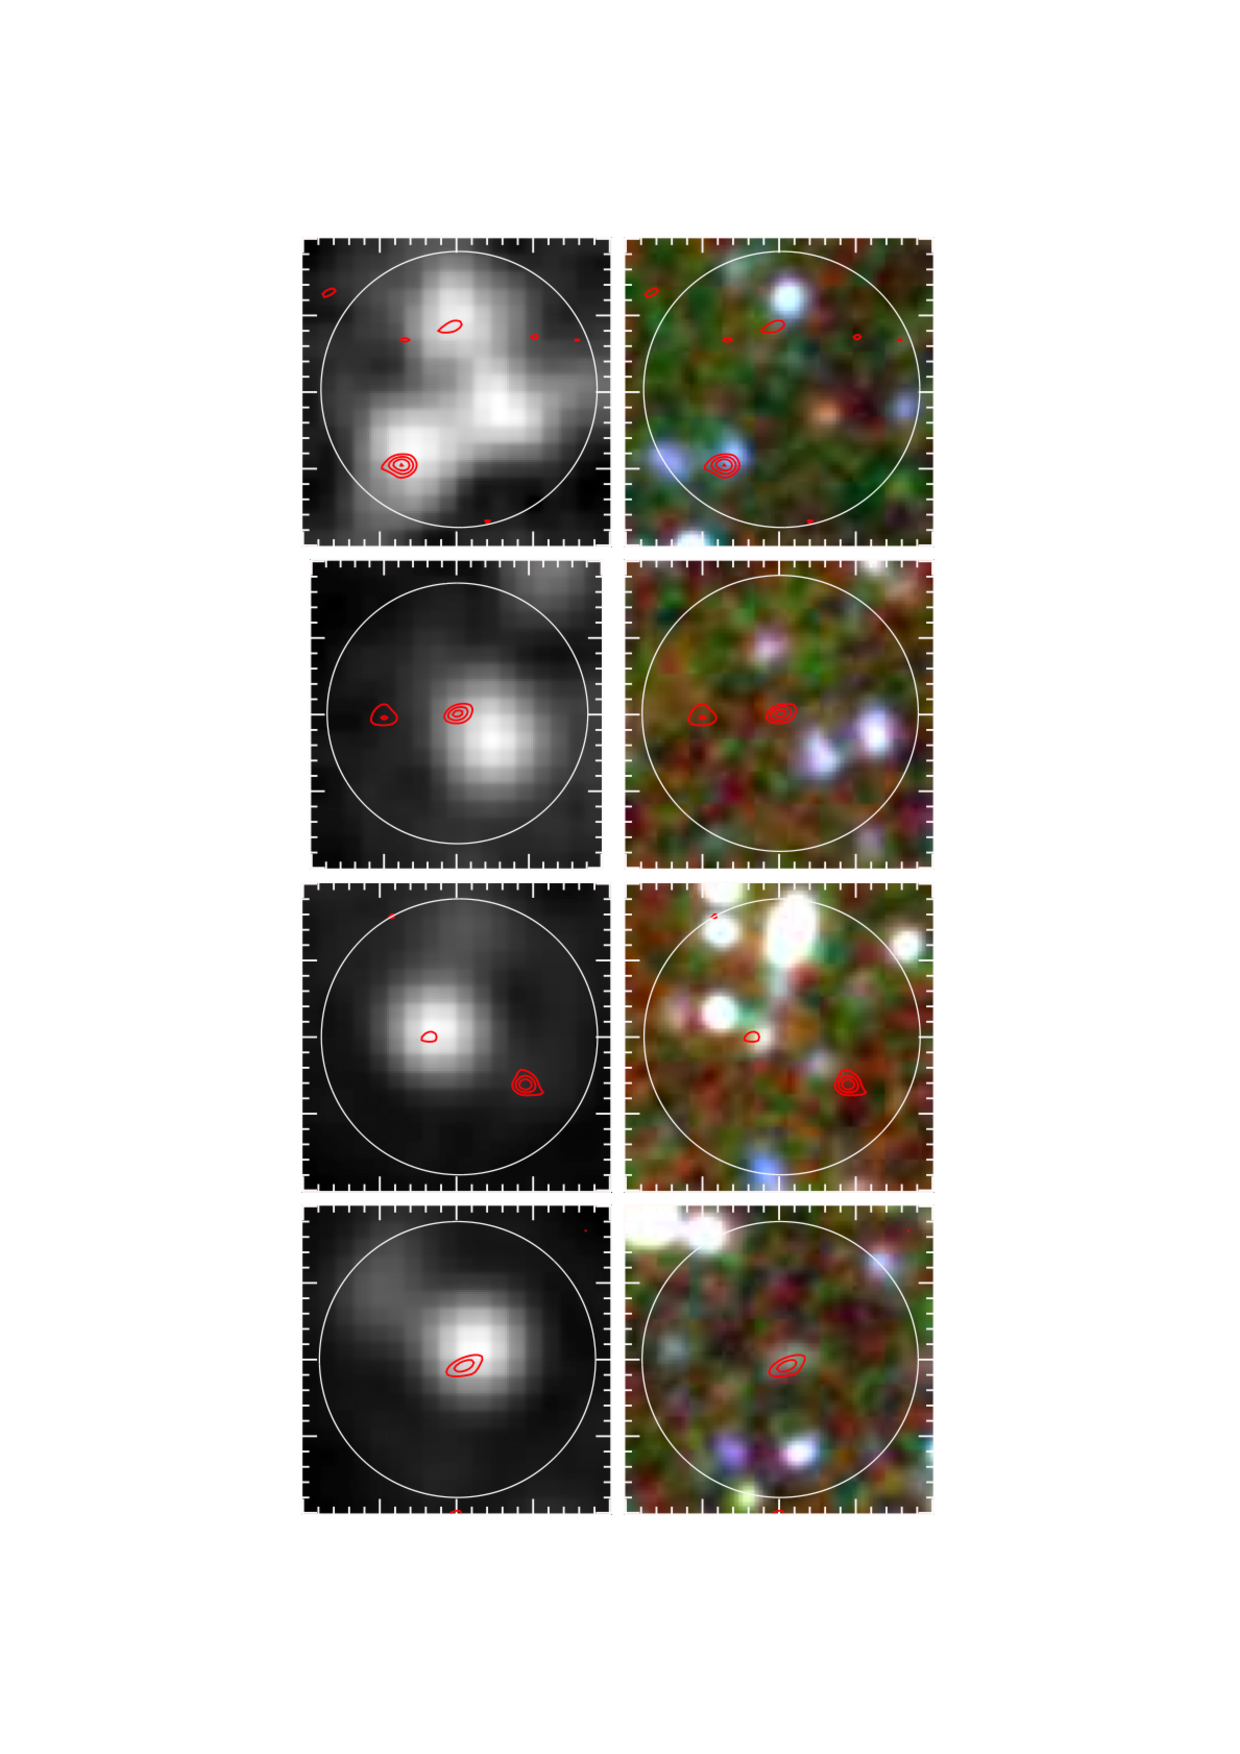
\includegraphics[width=5cm]{cfaless} 
\caption{ALMA 870-\micron\ contours (red) overlaid on
    24\micron\ (left) and {\it RIz} images (right) centered on four 
    250-\micron\ selected sources with ALMA data from the
    ALESS survey\protect\footnotemark (Hodge et al.\ 2013). The white circle is the 250-\micron\ beam. In some
    cases the 24\micron\ data are sufficient to identify the correct
    counterpart (e.g.\ bottom panel), but in others the 24\micron\ is
    complicated (e.g.\ top panel), or identifies the wrong counterpart or
    only one of several true counterparts (e.g.\ middle panels).}
\label{fig:cfaless}
\end{wrapfigure}

\protect\footnotetext{Only 13 \herschel\ 250-\micron\ selected sources
  have overlapping archival ALMA data from ALESS, with a further 25
  in various cycle 1 \& 2 programs. In many cases there is a
  large enough positional offset between the 250\micron\ centroid and
  the ALMA pointing center that faint counterparts outside of the ALMA
  primary beam may be missed. Though these data are informative as in
  Figure~\ref{fig:cfaless}, the small number of sources with
  overlapping data within the primary beam means that they are
  insufficient to achieve our science goals.}

The simplest approaches to the identification problem have assumed one high resolution counterpart is responsible for each \herschel-SPIRE source and have used statistical methods to make the identification (e.g.\ Smith et al.\ 2010; Fleuren \ea\
2012; Kim \ea\ 2012). 

These approaches provide incomplete identifications (40--80\%), are biased (depending on the wavelength of the matched catalogue), and are sometimes wrong, often due to the fact that one \herschel-SPIRE source is actually a combination of multiple galaxies (e.g. Figures \ref{fig:cfaless} and \ref{fig:triplots}, see e.g.\ Hodge \ea\ 2013 for a
discussion). 

%

%%  {\bf Source blending in the \herschel-SPIRE beam:}
%%  %
%%  The large \herschel\ beam at 250\micron, coupled with the surface
%%  density of far-infrared bright galaxies (e.g.\ Oliver \ea\ 2010; Glenn
%%  \ea\ 2010) indicates that at least some of the sources are composed of
%%  flux from several galaxies. The components of these blended sources
%%  may be physically related (e.g.\ the early stages of a merger) or a
%%  random line-of-sight alignment of unassociated galaxies.  The effect
%%  of blending must be taken into account when analysing the number
%%  counts because blending effectively shifts sources from lower to
%%  higher flux bins. Measurement of the blending rate in 250\micron\
%%  \herschel\ sources, coupled with the redshifts of the individual
%%  components, can also provide information about the clustering and
%%  interaction rate in these systems. So far blending has only been
%%  serendipitously confirmed in a handful of individual \herschel\
%%  sources and as such the rate of occurrence is unknown.  ALMA
%%  interferometry of classic $\sim850$-\micron\ selected SMGs shows that
%%  blending is prevalent in those samples, with $\sim35\%$ of them being composed of
%%  multiple components (Hodge et al.\ 2013).

{\bf Providing robust identifiers:}
%

The \herschel-PACS observations (with a beam of $\sim$ 12\arcsec\ FWHM at 160\micron) are ideal for providing identifications with the  \herschel-SPIRE sources as they are higher resolution. Where \herschel-PACS is to shallow, or there is no coverage, other high resolution wavelength data can be used to provide identifications. With over 70 square degrees of deep imaging data, \spitzer-24 \micron\ can be used for this purpose. 

However, since 24\micron\ samples wavelengths shorter than the peak of the dust SED, identifications are biased against galaxies with cooler (i.e.\ red) apparent submillimeter SEDs, which preferentially affects those at
high redshifts ( e.g.\ Pope et al.\ 2010; Dowell et al.\ 2013). Only with both 24\micron\ and 870\micron\ data from ALMA do we get a full unbiased list of potential counterparts to the \herschel-SPIRE sources.

This problem has been shown in other ALMA observing programs such as Bussmann et al. 2014, which we illustrate in Figure \ref{fig:triplots}. By using HELP's probabilistic deblender, XID+ (Hurley et al. in prep.) we can get the full posterior distribution of possible \herschel-SPIRE fluxes for a 24\micron\ counterpart and three ALMA 870 \micron\ counterparts for the target HADFS04. When only 24\micron\ counterparts or ALMA 870 \micron\ counterparts are considered, the deblended \herschel-SPIRE 250 micron fluxes are significantly different from when all are properly accounted for.

%An alternative approach towards characterising the 250\micron\ CIB is
%to use galaxies detected at shorter wavelengths (e.g. 24\, 100\, 160 \micron), as
%priors to trace galaxies that may contribute to the CIB (e.g.\
%B\'ethermin et al.\ 2012; Viero et al.\ 2013). This approach has
%yielded useful results, however the prior list of galaxies is incomplete due to the . Since 24\micron\
%samples wavelengths shorter than the peak of the dust SED, this
%incompleteness is biased against galaxies with cooler (i.e.\ red) apparent
%submillimeter SEDs, which preferentially affects those at
%high redshifts ( e.g.\ Pope et al.\ 2010; Dowell et al.\ 2013). Therefore, although these
%approaches are useful, to complete the samples in these studies, and recover the cooler
%submillimeter emitting galaxies, observations are required at longer
%wavelengths, at resolutions that, for statistically meaningful samples, can only be provided by
%the sensitive interferometric abilities of ALMA. The need for ALMA observations in such cases has already been highlighted in Bussmann \ea\  (submitted), where it has been shown that there are distinct ALMA sources close to 24\micron sources such that flux estimates alter substantially when taking into account the high redshift counterparts (e.g. Figure \ref{fig:triplots}).


%However, only 40--80\% of sources are statistically identified (depending
%on wavelength and depth of the matched catalogue), so the nature
%of the remaining 20--60\% cannot be determined. The unidentified
%sources are not a random subset of the parent sample, they are likely to be the highest-redshift galaxies, which are faint at optical, near- and mid-infrared, and radio wavelengths, and may not be detected
%even in deep imaging.

%420,000 SPIRE blobs in 1000 square degrees. Over 70 square degrees 30,000 we have 24micron data..
%600 rock solid identifications
%double 

{\bf This proposal:}
%

Our fundamental goal is to obtain a complete set of robust identifications for all sources above the nominal confusion limit of \herschel-SPIRE at 250 \micron. This gold standard will then be a representative benchmark for all past and future studies dependent on the 420,000 sources above the confusion limit in \herschel-SPIRE's 1000 square degree legacy.

We have chosen a flux limit of $S_{250}>35$\,mJy, which is $\sim 6\sigma$, above confusion noise (Nguyen et al. 2010) and comfortably brighter than the 40 beams per source confusion limit (Oliver et al. 2010). 

In order to provide a representative sample across the variety of source colours and redshifts, we require a sample size of $>$ 600, allowing subdivision into $\sim$ 8$\times$8 bins with $\sim$10 sources in each bin.

This corresponds to an area of $\sim$ 1.2 $\times$ 1.2 degrees. We have chosen the COSMOS field due to the depth of the PACS data which ensures the best and most complete preexisting identifications for 70\% of our sample.

The COSMOS field is also the most well-studied extragalactic survey field of this size, with outstanding auxiliary data, including deep optical and
near-infrared photometry and spectroscopy, and mid-infrared and radio
photometry. This will allow us to determine the multi-wavelength properties of the identified counterparts to the depth of ``normal"($\sim$ L*) galaxy population through a large fraction of cosmic history. 

From the COSMOS field, we have a complete sample of 612 sources, of which 183 have no \herschel-PACS identifications. These sources are likely to be the higher redshift objects for which identification may only be possible with ALMA. We will perform 870-\micron\ observations to robustly identify the counterparts to these unidentified sources.

Given the short exposure times and the overheads associated with ALMA observations, we can efficiently add additional targets. We will therefore perform 870-\micron\ observations for a control sample of 117 objects, adding $<$20\% to the observing time. Our control sample has been carefully selected from the sources with PACS identifications and uniformly samples the $\log (S_{250 \mathrm{\mu m}}/S_{100\mathrm{\mu m}})$ colours. This control sample will represent 27\% of the PACS identifications and will be used to assess their validity and produce gains towards the understanding of sources that are not sampled (e.g. in other fields). %
%subscript mcirons
%

{\bf Immediate Science Goals:}
The immediate science goal is to understand the multiplicity of \herschel-SPIRE sources, in order to address the issues raised in Hodge et al. 2013 and Cowley et al. 2015.

Our second science goal will be to provide a training set for \herschel-SPIREs 1000 deg.$^2$ of data. Given this gold standard sample, we can mimic the issues related to all \herschel\ data, such as those fields where only $r$-band or 24 \micron\ MIPS data is available.

Thirdly, we will use our sample of 612 \herschel-SPIRE with robust identifications, and the wealth of available ancillary data, to build and fit
stellar SEDs. These will be used to measure photometric redshifts and
stellar masses of the 250-\micron\ selected galaxies (e.g.\ Wardlow et
al.\ 2011) as well as providing the infrared
luminosity functions and contribution to the star-formation rate
density of 250-\micron\ selected galaxies. The redshifts, stellar
masses, dust temperature and infrared luminosity functions will be
compared with other galaxy populations at both high and low redshift
(e.g.\ 870-\micron\ selected galaxies, {\it BzK} galaxies, local
early-type galaxies) and predictions from galaxy formation theories
(e.g.\ B\'ethermin et al.\ 2011, Hayward et al.\ 2012 ) to place the
250-\micron\ selected galaxies in the context of Universal galaxy
evolution.

As Co-Is of the proposal are core members of HerMES and HELP, we will exploit their expertise and tools to get a full handle on the degeneracies in \herschel-SPIRE fluxes, introduced by considering multiple counterparts to a SPIRE source (e.g. Figure \ref{fig:triplots}).

%%  Targets (probably 60-80):\\
%%  UDS, COSMOS or ECDFS\\
%%  $S250\ge30mJy$ (or 35mJy if in COSMOS). This means everything is
%%  $>5\sigma$.\\
%%  Ensure a range of 250 fluxes and 250-350, 250-500 and 250-24um
%%  colours in the subsample of targets selected. \bf -- OR -- } Sampling
%%  f24, f850 plane, i.e. read-off SPIRE beam convolved f24 and f850 maps
%%  (as produced by Charlotte above) the (f24,f850)$_i$ for every i source
%%  in f250 catalogue.  Plot (f24,f850) and then evenly sample this space. \\
%%  Exclude local resolved late-type spirals.\\
%%  Check ancillary data coverage\\
%%  Check duplications


\hspace{0.2cm}
{\bf Observing strategy:}
We will observe the 300 250-\micron\ selected targets in continuum
mode in ALMA band 7, centering the observations at 343\,GHz
(873\micron). 
%
The requested resolution of 1'' is sufficient to positionally match
ALMA data to the existing imaging in the COSMOS field. The target depth of 0.2mJy/beam
is required to solidly detect the galaxies at $\ge5\sigma$ even in
cases where the 250-\micron\ selected source is a blend of 2--3
galaxies. The ALMA band 7 primary beam matches the resolution of
\herschel\ at 250\micron, such that we do not have to be concerned
with potential counterparts residing outside of the spatial area to
which ALMA is sensitive.


\begin{wrapfigure}{r}{0.48\textwidth}
\centering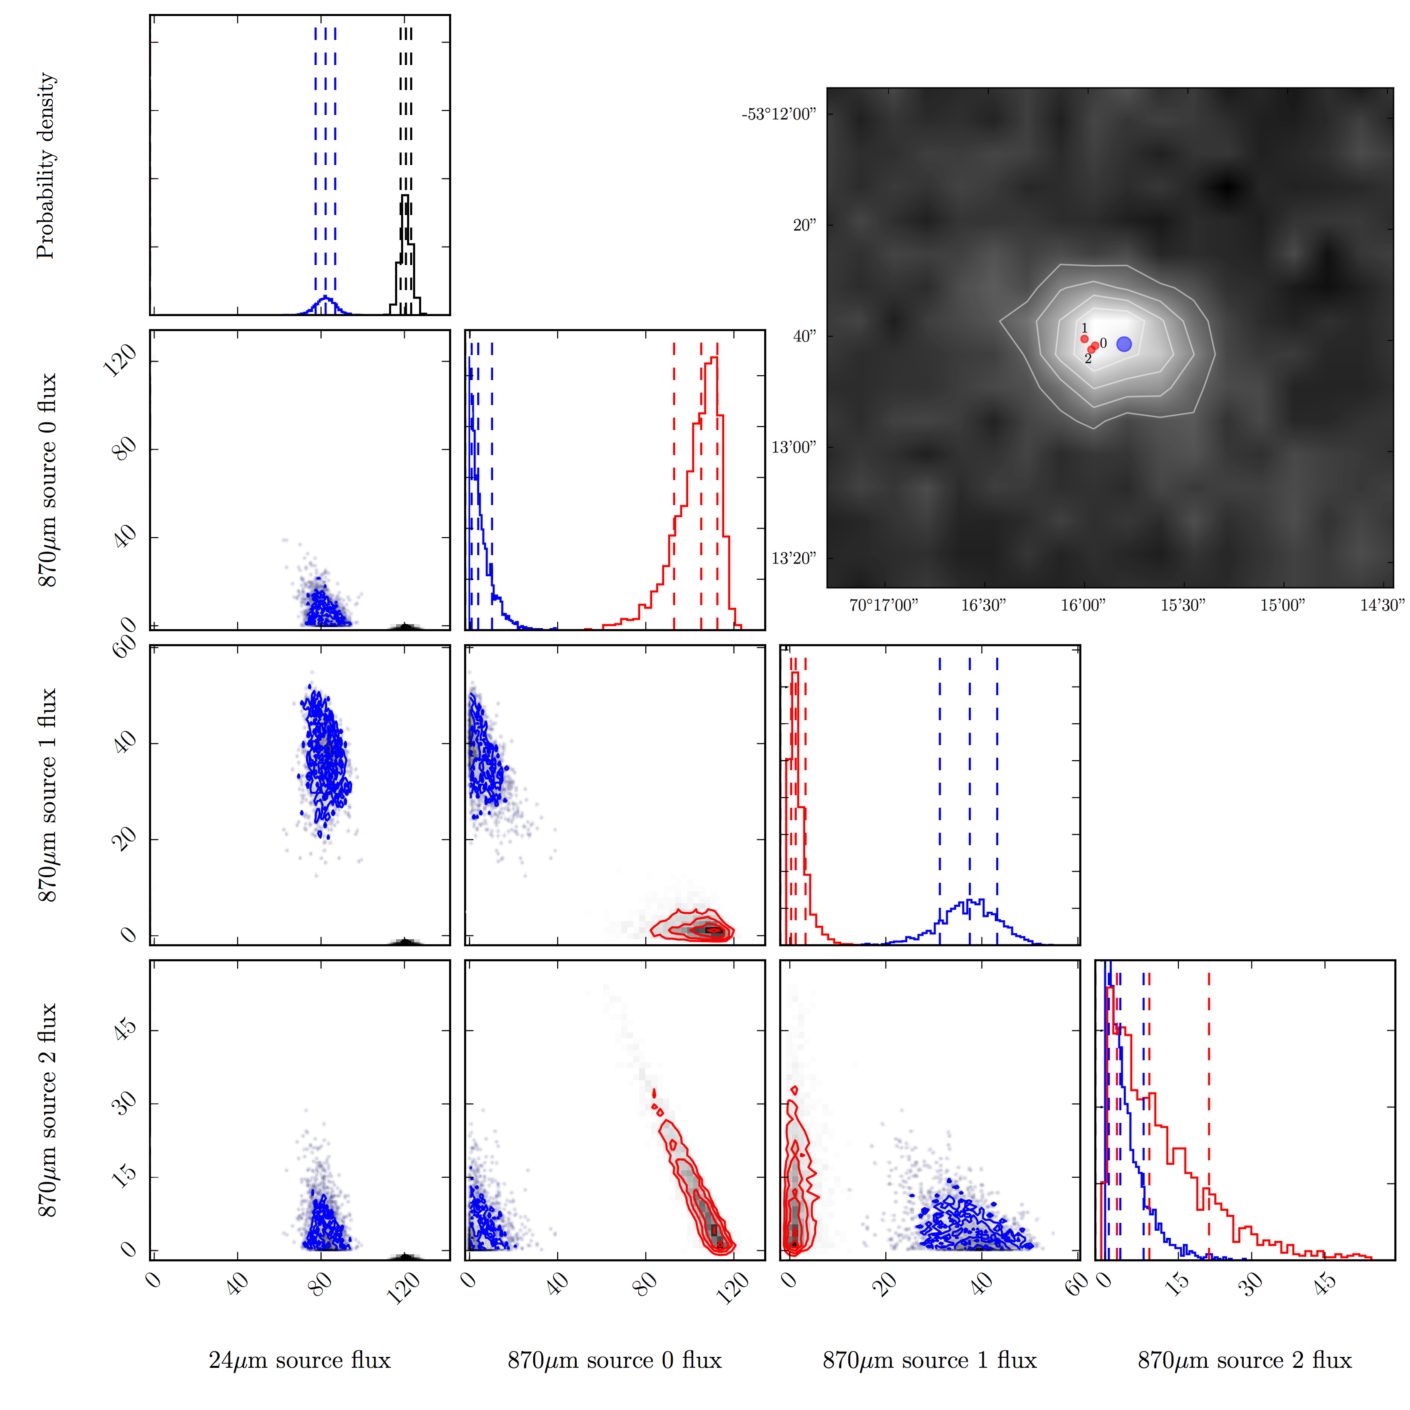
\includegraphics[width=9cm]{250XID+beta_ADFS04_merged_edit.pdf} 
\caption{An example of how the deblended \herschel-SPIRE 250\micron\ fluxes differ for HADFS04 (Bussmann et al. 2015), when considering only the 24\micron\ source (black), only the ALMA positions (red) and when both are correctly included (blue). Dashed lines represent 15th, 50th and 84th percentiles in probability density plots. Deblending is done with XID+, software being developed as part of HELP (Hurley \ea\  in prep.)}
\label{fig:triplots}
\end{wrapfigure}

870\,\micron\ fluxes are predicted by fitting various SED
templates (Efstathiou et al.\ 2000; Xu et al.\
2003; Poletta et al.\ 2007) to the \herschel\ photometry, leaving
redshift as a free parameter. The expectations from the SED fits are
consistent with the fluxes that are measured from coincident ALMA data for a handful of cases
in ECDFS (Figure~\ref{fig:cfaless}). 

%%   Enter the scientific justification here, together with any figures and tables that you judge necessary.
%%    
%%   %-----------------------------Figure Start---------------------------
%%   \begin{figure}[tbh]
%%   % The 'scale' parameter below allows you to scale the figure so that it fits within the page. In this case the figure was scaled to 20% of its original size.
%%   \includegraphics[scale=0.2]{CO_velfield.png}
%%   \caption{\em{The CO(1-0) velocity field of NGC\,3256, with contours 
%%   of the total line emission map overlaid (ALMA Science Verification Data).
%%   }}
%%   \end{figure}
%%   %-----------------------------Figure End------------------------------
%%   
%%   %-----------------------------Table Start-----------------------------
%%   \begin{table}[tbh]
%%   \begin{center}
%%   \caption[]{\em{Here we show the continuum sensitivity required per band.}}
%%   \begin{tabular}{cc}
%%   \hline \noalign {\smallskip}
%%   Frequency (GHz) & Sensitivity (mJy) \\
%%   \hline \noalign {\smallskip}
%%   100 & 0.01 \\
%%   300 & 0.10 \\
%%   %\hline \noalign {\smallskip}
%%   \end{tabular}
%%   \end{center}
%%   \end{table}
%%   %-----------------------------Table End ------------------------------
%%   
%%   You can structure the scientific justification using the two subsections below (optional).

%%  \subsection{Scientific rationale}

% Please describe the scientific background of the project,
% pertinent references and previous work relevant to this 
% proposal.

%%  \subsection{Immediate objectives}

% Please describe the observations to be made and their specific
% purpose, with a clear explanation of the need for, and 
% appropriateness of, ALMA Cycle 1 data.  

%%%%%%%%%%%%%%%%%%%%%%%%%%%%%
%% Potential for Publicity %%
%%%%%%%%%%%%%%%%%%%%%%%%%%%%%
{\large{\bf 2 Potential for Publicity}}

% Here, include a brief statement on the potential of your proposal
% to generate publicity based on the scientific results to be obtained.

% ALMA is the only (sub)millimeter facility that can achieve sufficient
% resolution and sensitivity for our science goals. Several other
% observatories can achieve the necessary resolution, but ALMA is the
% only one with the sensitivity to target a statistically significant
% and representative sample of 250-\micron\ selected sources, as we
% require here.
% By pinpointing the position of the submillimeter emission in a
% representative sample of 250-\micron\ selected sources we will
% isolate, for the first time, the systems at the peak of the Cosmic
% Infrared Background.
% The targets are located in a field with deep,
% complimentary radio, near- and mid-infrared, and optical data, which
% will provide a multiwavelength view of the ALMA-identified
% counterparts.  

As well as providing a first detailed look at the
systems contributing to the Cosmic Infrared Background, the proposed
data will enable us to link imaging from the UV, optical, near-, mid-
and far-infrared, and radio. We will produce montages of these
high-redshift galaxies, which will both reveal their nature and be
visually appealing. The resulting images will be worthy of public release,
thanks to the combination of ALMA and existing
multi-wavelength data.  We
will work closely with the ALMA Education and Public Outreach team to
prepare these. Since this project involves \herschel-selected sources,
we will also have \herschel\ ESA and NASA outreach resources at our
disposal. The results will be of interest to the general astronomical
community and will effectively demonstrate the unique power of ALMA to
potential users and to the public.  We will disseminate the results to
the astronomical community via publications and presentations at
conferences and seminars.


%%%%%%%%%%%%%%%%%%%%%%%%
%% References section: %
%%%%%%%%%%%%%%%%%%%%%%%%
{\large{\bf 3 References:}}

B\'ethermin et al.\ 2010, A\&A, 512, 78 $\bullet$
B\'ethermin et al.\ 2011, A\&A, 529, 4 $\bullet$ 
B\'ethermin et al.\ 2012, A\&A, 542, 58 $\bullet$
Burgarella et al. \ 2013 A\&A, 554, 70 $\bullet$
Bussmann et al. \ arXiv:1504.05256 $\bullet$
Berta et al.\ 2011, A\&A, 532, 4 $\bullet$
Cooray et al. \ 2010, A\&A 518, 22, $\bullet$
Cowley et al. arxiv:1504.04516 $\bullet$
Dole et al.\ 2006, A\&A, 451, 417 $\bullet$
Dowell et al.\ 2013, arXiv:1310.7583 $\bullet$
Efstathiou et al.\ 2000, MNRAS, 313, 734 $\bullet$
Elbaz et al. \ 2011, A\&A, 533, 119 $\bullet$
Fixsen et al.\ 1998, ApJ, 508, 123 $\bullet$
Fleuren et al.\ 2012, MNRAS, 423, 2407 $\bullet$
Glenn et al.\ 2010, MNRAS, 409, 109 $\bullet$
Hauser \& Dwek, 2001, ARA\&A, 39, 249 $\bullet$
Hayward et al.\ 2012, 424, 951 $\bullet$
Hodge et al.\ 2013, ApJ, 768, 91 $\bullet$
Hurley et al. \ in prep. $\bullet$
Kim et al.\ 2012, ApJ, 756, 28 $\bullet$
Lagache et al.\ 1999, A\&A, 344, 322 $\bullet$
Nguyen et al. 2010, A\&A, 518, L5 $\bullet$
Oliver et al.\ 2010, A\&A, 518, L21 $\bullet$
Oliver et al.\ 2012, MNRAS, 424, 1614 $\bullet$
Papovich et al.\ 2004, ApJS, 154, 70 $\bullet$
Poletta et al.\ 2007, ApJ, 663, 81 $\bullet$
Pope et al.\ 2010, ApJ, 715, 171 $\bullet$
Puget et al.\ 1996, A\&A, 308, L5 $\bullet$
Roseboom et al.\ 2010, MNRAS, 409, 48 $\bullet$
Smith et al.\ 2010, MNRAS, 416, 857 $\bullet$
Smol\^ci\'c et al.\ 2012, A\&A, 548, 4 $\bullet$
Simpson et al.\ 2013. arXiv:1310.6363 $\bullet$
Swinbank et al.\ 2013, arXiv:1310.6362 $\bullet$
Viero et al.\ 2013, ApJ, 772, 77 $\bullet$
Wardlow, et al.\ 2011, MNRAS, 415, 1479 $\bullet$
Xu et al.\ 2003, ApJ 587, 90 $\bullet$



%%%%%%%%%%%%%%%%%%%%%%%%%%%
%%%%% End of document %%%%%
%%%%%%%%%%%%%%%%%%%%%%%%%%%

\end{document}

